\documentclass[landscape]{article}

\usepackage[top=2.5cm, left = 1.5cm,right=1.5cm,bottom=1cm]{geometry}
\usepackage{tikz}

\newcommand{\cellheight}{17}
\pagestyle{empty}
\begin{document}

\centering
%Month \rule{3cm}{1pt}\\[1cm]

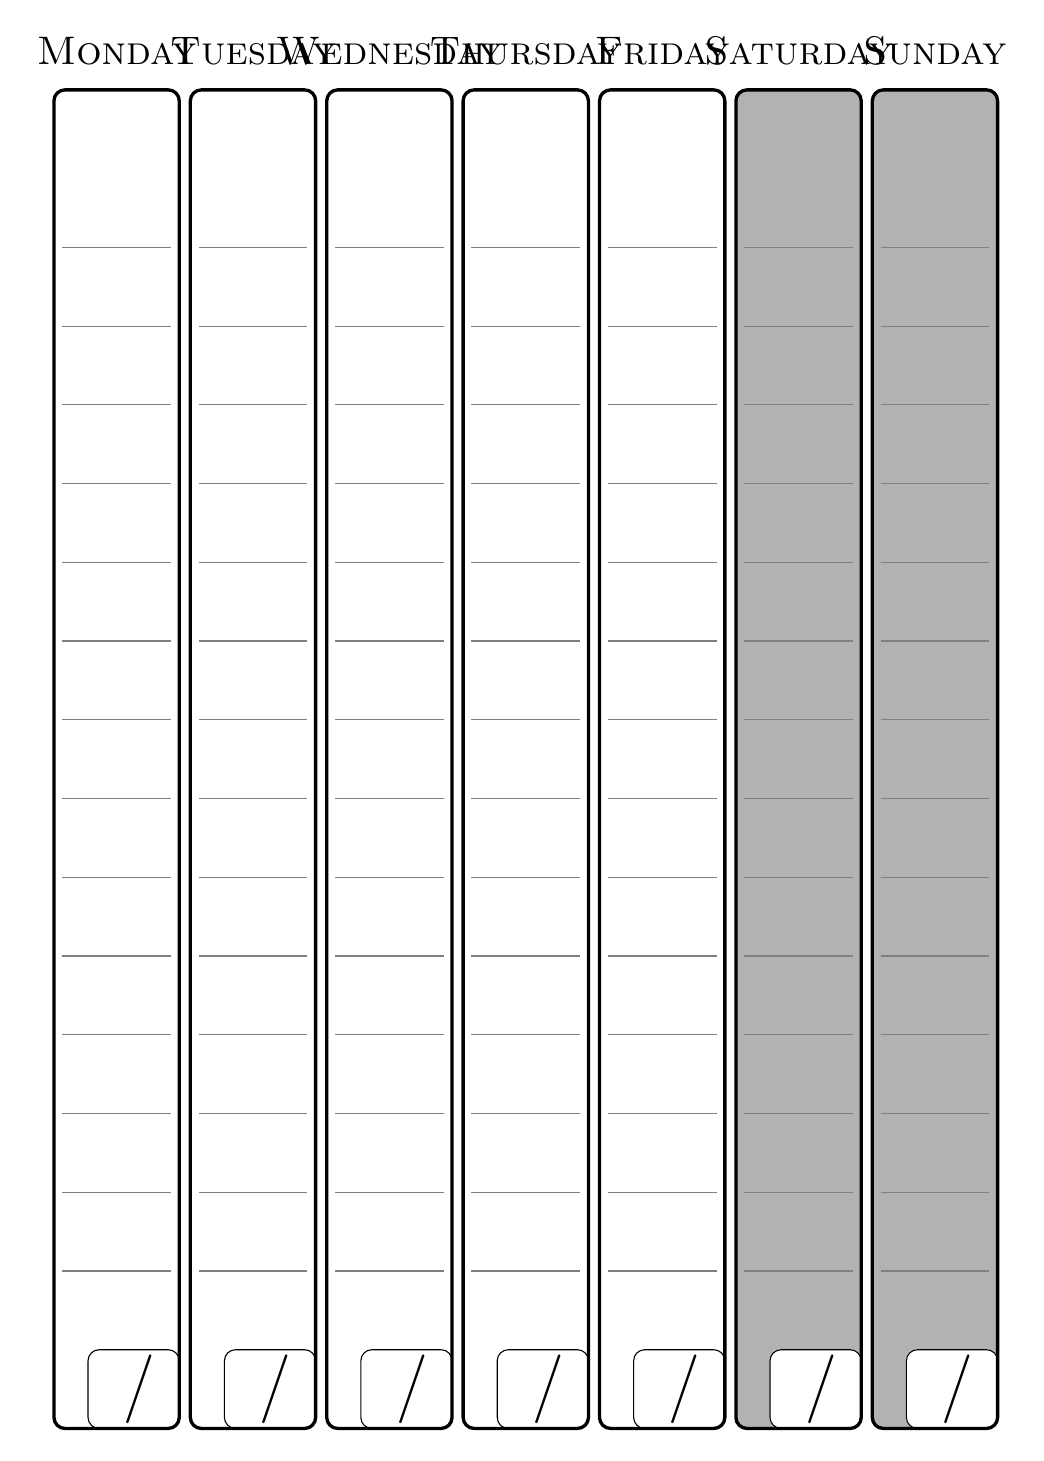
\begin{tikzpicture}
	
	\foreach \i/\D in {5,6}
	{	
		\draw[rounded corners, fill, black!30] (\i*\linewidth/7+.2em,0) rectangle (\i*\linewidth/7+\linewidth/7-.2em,\cellheight); 
		\draw[rounded corners, fill, white] (\i*\linewidth/7 + \linewidth/28+.2em,0) rectangle (\i*\linewidth/7+\linewidth/7-.2em,1);
	}
	
	\foreach \i/\D in {0/Monday,1/Tuesday,2/Wednesday,3/Thursday,4/Friday,5/Saturday,6/Sunday}
	{	
		\node[] () at (\i*\linewidth/7+\linewidth/14,\cellheight+.5) {{\Large \sc \D}};
		\draw[rounded corners, very thick] (\i*\linewidth/7+.2em,0) rectangle (\i*\linewidth/7+\linewidth/7-.2em,\cellheight); 
		\draw[rounded corners] (\i*\linewidth/7 + \linewidth/28+.2em,0) rectangle (\i*\linewidth/7+\linewidth/7-.2em,1);
		\node[] () at (\i*\linewidth/7 + 2.5*\linewidth/28 + .2em,.5) {{\Huge /}};
		\foreach \y in {2,...,15}
		{
			\draw[gray] (\i*\linewidth/7+.5em,\y) -- (\i*\linewidth/7+\linewidth/7-.5em,\y);
		}
	}

\end{tikzpicture}


\end{document}